\subsection{BÀI TẬP TRẮC NGHIỆM}
\ind{PHẦN I.} \inden{Câu trắc nghiệm nhiều phương án lựa chọn. Mỗi câu hỏi học sinh chỉ chọn một phương án.}\\
\setcounter{ex}{0}
\Opensolutionfile{ans}[ans/0H4-B4-1]

\begin{ex}%[0H1B4-3]
	Trong mặt phẳng tọa độ $Oxy$. Khẳng định nào dưới đây \textbf{sai}?
	\choice
	{Điểm $A$ nằm trên trục tung thì có hoành độ bằng 0}
	{Tọa độ của điểm $A$ là tọa độ của vectơ $\overrightarrow{OA}$}
	{\True Điểm $A$ nằm ở góc phần tư thứ hai thì có hoành độ dương}
	{Điểm $A$ nằm trên trục hoành thì có tung độ bằng 0}
	\loigiai{
		Điểm $A$ nằm ở góc phần tư thứ hai có hoành độ âm và tung độ dương.}
\end{ex}

\begin{ex}%[0H1B4-3]
	Trong hệ trục $(O; \overrightarrow{i}, \overrightarrow{j})$, tọa độ của vectơ $\overrightarrow{i} -\overrightarrow{j}$ là
	\choice
	{$(-1;1)$}
	{$(1;0)$}
	{$(0;1)$}
	{\True $(1;-1)$}
	\loigiai{
		Tọa độ của $\overrightarrow{i}-\overrightarrow{j}$ là $(1;-1)$.
	}
\end{ex}

\begin{ex}%[0H1Y4-3]
	Trong hệ trục toạ độ $Oxy$, cho hai điểm $A(2;-1)$, $B(4;3)$. Toạ độ của vectơ $\overrightarrow{AB}$ bằng
	\choice
	{\True $\overrightarrow{AB}=(2;4)$}
	{$\overrightarrow{AB}=(6;2)$}
	{$\overrightarrow{AB}=(-2;-4)$}
	{$\overrightarrow{AB}=(8;-3)$}
	\loigiai{
		$\overrightarrow{AB}=\left(4-2;3-(-1)\right)=(2;4)$
		.}
\end{ex}

\begin{ex}%[0H1B4-3]
	Trong mặt phẳng tọa độ $Oxy$, cho hai vectơ $\overrightarrow{OA} =2\overrightarrow{i} -\overrightarrow{j}$ và $\overrightarrow{OB} =5\overrightarrow{i} +2\overrightarrow{j}$. Tính tọa độ của vectơ $\overrightarrow{AB}$.
	\choice
	{$\overrightarrow{AB} =(-3;-3) $}
	{$\overrightarrow{AB} =(2;-1) $}
	{\True $\overrightarrow{AB} =(3;3)$}
	{$\overrightarrow{AB} =(7;1)$}
	\loigiai{
		Ta có $\overrightarrow{AB}=\overrightarrow{OB}-\overrightarrow{OA}=3\overrightarrow{i}+3\overrightarrow{j}\Rightarrow \overrightarrow{AB}=(3;3)$.
	}
\end{ex}

\begin{ex}%[0H1Y4-3]
	Cho tam giác $ABC$. Gọi $M$, $N$, $P$ lần lượt là trung điểm của $BC$, $CA$, $AB$. Biết $A(1;3)$, $B(-3;3)$, $C(8;0)$. Giá trị của $x_M+x_N+x_P$ bằng
	\choice
	{$1$}
	{\True $6$}
	{$2$}
	{$3$}
	\loigiai{
		Ta có $x_M=\dfrac{x_B+x_C}{2}=\dfrac{-3+8}{2}=\dfrac{5}{2}$, $x_N=\dfrac{x_A+x_C}{2}=\dfrac{1+8}{2}=\dfrac{9}{2}$, $x_P=\dfrac{x_A+x_B}{2}=\dfrac{1-3}{2}=-1$.\\
		Vậy $x_M+x_N+x_P=\dfrac{5}{2}+\dfrac{9}{2}-1=6$.
	}
\end{ex}

\begin{ex}%[0H1B4-3]
	Trong mặt phẳng $Oxy$, cho tam giác $EHF$ có $E(-1;3)$, $H(3;-4)$, $F(4;2)$. Tìm tọa độ trọng tâm $G$ của tam giác $EHF$.
	\choice
	{$G\left(\dfrac{8}{3};\dfrac{1}{3}\right)$}
	{\True $G\left(2;\dfrac{1}{3}\right)$}
	{$G\left(\dfrac{8}{3};3\right)$}
	{$G(2;3)$}
	\loigiai{
		$G$ là trọng tâm của tam giác $EHF$ nên $\heva{&x_G=\dfrac{x_E+x_F+x_H}{3}=\dfrac{-1+3+4}{3}=2 \\& y_G=\dfrac{y_E+y_F+y_H}{3}=\dfrac{3-4+2}{3}=\dfrac{1}{3}}\Rightarrow G\left(2;\dfrac{1}{3}\right)$.}
	%<MyLT>
\end{ex}

\begin{ex}%[0H1B4-3]
	Trong mặt phẳng tọa độ $Oxy$, cho hình bình hành $OABC$ có $B(-6;12)$. Tìm tọa độ tâm $I$ của hình bình hành $OABC$.
	\choice
	{$I(1;-4)$}
	{\True $I(-3;6)$}
	{$I(3;-6)$}
	{$I(-1;4)$}
	\loigiai
	{
		Tâm $I$ của hình bình hành $OABC$ là trung điểm của $OB$. Vậy $I(-3;6)$.
	}
\end{ex}

\begin{ex}%[0H1Y4-3]
	Trong mặt phẳng với hệ tọa độ $Oxy$, cho ba điểm $A(1;2), B(-2;-3)$ và $G(-1;-1)$. Tìm tọa độ điểm $C$ sao cho $G$ là trọng tâm tam giác $ABC$.
	\choice
	{$(1;-1)$}
	{$(2;-2)$}
	{$(-1;1)$}
	{\True $(-2;-2)$}
	\loigiai{
		Ta có: $G$ là trọng tâm tam giác $ABC$ nên $\heva{&x_G=\dfrac{x_A+x_B+x_C}{3} \\& y_G=\dfrac{y_A+y_B+y_C}{3}}\Leftrightarrow \heva{&-1=\dfrac{1-2+x_C}{3} \\& -1=\dfrac{2-3+y_C}{3}}\Leftrightarrow \heva{&x_C=-2 \\& y_C=-2.}$\\
		Vậy $C(-2;-2)$.}
	%<MyLT>
\end{ex}

\begin{ex}%[0H1B4-3]
	Trong mặt phẳng $Oxy$, cho $\triangle MNP$ có $M(1;-1)$, $N(5;-3)$ và $P$ thuộc trục $Oy$, trọng tâm $G$ của $\triangle MNP$ nằm trên trục $Ox$. Tọa độ điểm $P$ là
	\choice
	{$ (0;2) $}
	{$ (2;4) $}
	{\True $ (2;0) $}
	{$ (0;4) $}
	\loigiai{
		Vì $P \in Oy,~G \in  Ox$ nên $P(0;y_P),~G(x_G;0)$. Mặt khác $G$ là trọng tâm $\triangle MNP$ nên ta có \\
		$\heva{& x_G=\dfrac{1+5+0}{3}\\& 0=\dfrac{-1+(-3)+x_P}{3}} \Rightarrow x_P=4$.
		Vậy $P(0;4)$ là điểm cần tìm.
	}
\end{ex}

\begin{ex}%Câu 1
	\immini[thm]{Sự chuyển động của một tàu thuỷ được thể hiện trên một mặt phẳng tọa độ như sau: Tàu khởi hành từ vị trí $ A\left(0;1\right)$ chuyển động thẳng đều với vận tốc (tính theo giờ) được biểu thị bởi vectơ $\vec v=\left(2;4\right)$. Xác định vị trí $B$ của tàu (trên mặt phẳng toạ độ) tại thời điểm sau khi khởi hành $ 2,5$ giờ.
		\choice
		{$ B\left(4,5;6,5\right)$}
		{$ B\left(5;9\right)$}
		{\True $ B\left(5;11\right)$}
		{$ B\left(2;4\right)$}
	}{
		\begin{tikzpicture}[smooth,samples=300,scale=0.8,>=stealth,font=\footnotesize]
			\draw[line width=0.15pt,dashed] (-0.5,-0.5) grid (5.5,5.5);
			\draw[->] (-0.8,0)--(5.5,0) node[below]{$x$};
			\draw[->] (0,-0.5)--(0,5.5) node[right]{$y$};
			\draw (0,0) node[above left]{$O$};
			\draw[fill=black] (0,1) circle(1.5pt)node[above left]{$A$};
			\draw[->] (0,0)--(2,4)node[below right]{$\vec{v}$};
			%\node[right] at (2,2.4) {$2$};
	\end{tikzpicture}}
	\loigiai{
		Trên mặt phẳng tọa độ $ Oxy$, gọi $ B\left(x;y\right)$ là điểm biểu diễn vị trí của tàu tại thời điểm sau khi khởi hành $ 2,5$ giờ. 	Do tàu chuyển động thẳng đều từ $ A$ đến $ B$ với vận tốc (tính theo giờ) được biểu thị bởi vectơ $\vec v=\left(2;4\right)$ nên cứ sau mỗi giờ tàu sẽ di chuyển được một quãng đường bằng $\left|\overrightarrow v\right|$ .\\
		Khi đó: $\overrightarrow{AB}=2,5.\vec v\Leftrightarrow\left\{{\begin{array}{*{20}{l}}
				{x=2,5\cdot 2}\\
				{y-1=2,5\cdot 4}
		\end{array}}\right.\Leftrightarrow\left\{{\begin{array}{*{20}{l}}
				{x=5}\\
				{y=11}
		\end{array}}\right.$.\\
		Vậy sau $ 2,5$ giờ tàu đến vị trí điểm $ B\left(5;11\right)$.}
\end{ex}


\begin{ex}%[0H1B4-5]
	Trong mặt phẳng tọa độ $Oxy$ cho vectơ $\overrightarrow{a} =(-5;0)$, $\overrightarrow{b} =(4;m)$. Tìm $m$ sao cho hai vectơ $\overrightarrow{a}$ và $\overrightarrow{b}$ cùng phương.
	\choice
	{$m=-5$}
	{$m=-1$}
	{\True $m=0$}
	{$m=4$}
	\loigiai{
		Hai vectơ đã cho cùng phương khi và chỉ khi $-5\cdot m-0\cdot 4=0\Leftrightarrow m=0.$
	}
\end{ex}

\begin{ex}
	Trong mặt phẳng tọa độ ${Oxy}$, cho hai véctơ $\overrightarrow{u}=(-8;-1)$ và $\overrightarrow{w}=(-7;-1)$. Tìm tọa độ véctơ ${\overrightarrow{u}+\overrightarrow{w}}$.\\ 
	\choice
	{ ${\overrightarrow{u}+\overrightarrow{w}=(1;0)}$ }
	{ ${\overrightarrow{u}+\overrightarrow{w}=(56;1)}$ }
	{ \True ${\overrightarrow{u}+\overrightarrow{w}= (-15;-2)}$ }
	{ ${\overrightarrow{u}+\overrightarrow{w}=(-9;-8)}$ }
	\loigiai{ 
		${\overrightarrow{u}+\overrightarrow{w}}=(-15;-2)$. 
}\end{ex}

\begin{ex}%[0H1B4-3]
	Trong mặt phẳng tọa độ $Oxy$, cho $\overrightarrow{a}=(1;2)$, $\overrightarrow{b}=(-2;1)$, $\overrightarrow{c}=(3;-1)$. Tính tọa độ của vectơ $\overrightarrow{x}=2\overrightarrow{a}+\overrightarrow{b}-\overrightarrow{c}$.
	\choice
	{$(3;6)$}
	{\True $(-3;6)$}
	{$(-3;-6)$}
	{$(3;-6)$}
	\loigiai{
		$\overrightarrow{x}=(2-2-3;4+1+1)=(-3;6)$.
	}
\end{ex}

\begin{ex}%[0H1B4-4]
	Cho ba vectơ $\overrightarrow{a}=(2;1)$, $\overrightarrow{b}=(3;4)$, $\overrightarrow{c}=(7;2)$. Giá trị của $k$, $h$ để $\overrightarrow{c}=k\overrightarrow{a}+h\overrightarrow{b}$ là
	\haicot
	{\True $k=4{,}4;h=-0{,}6$}
	{$k=3{,4};h=-0{,}2$}
	{$k=4{,}6; h=-5{,}1$}
	{$k=2{,}5;h=-1{,}3$}
	\loigiai{
		Ta có hệ
		$$\heva{&2k+3h=7\\&k+4h=2}\Leftrightarrow\heva{&k=4{,}4\\&h=-0{,}6.}$$
		Vậy $k=4{,}4;h=-0{,}6$.
	}
\end{ex}


\begin{ex}%[0H1B4-3]
	Trong mặt phẳng tọa độ $Oxy$, cho các điểm $A(1;4)$, $B(-3;2)$, $C(-3;-5)$, $M(x;y)$ thỏa mãn $\overrightarrow{MA}+\overrightarrow{MB}-2\overrightarrow{AC}=\overrightarrow{0}$. Khẳng định nào sau đây đúng?
	\choice
	{$y=-2x$}
	{$y=\dfrac{1}{3}x$}
	{$y=\dfrac{1}{4}x$}
	{\True $y=4x$}
	\loigiai{
		Ta có $\overrightarrow{MA}=(1-x;4-y)$, $\overrightarrow{MB}=(-3-x;2-y)$, $\overrightarrow{AC}=(-4;-9)$.\\
		Do đó $\overrightarrow{MA}+\overrightarrow{MB}-2\overrightarrow{AC}=\overrightarrow{0} \Leftrightarrow \heva{&1-x-3-x+8=0 \\& 4-y+2-y+18=0}\Leftrightarrow \heva{&x=3 \\& y=12}$. Suy ra $y=4x$.}
\end{ex}

\begin{ex}%[0H1B4-4]
	Trong hệ tọa độ $Oxy$, cho điểm $A(-1;1)$, $B(1;3)$, $C(-2;0)$. Khẳng định nào sau đây là \textbf{sai}?
	\choice
	{$A$, $B$, $C$ thẳng hàng}
	{\True $\overrightarrow{AB}=2\overrightarrow{AC}$}
	{$\overrightarrow{BA}=\dfrac{2}{3}\overrightarrow{BC}$}
	{$\overrightarrow{BA}+2\overrightarrow{CA}=\overrightarrow{0}$}
	\loigiai{
		Ta có $\overrightarrow{BA}=(-2;-2)$, $\overrightarrow{AC}=(-1;-1)$, $\overrightarrow{BC}=(-3;-3)$.\\
		Ta thấy $\overrightarrow{BA}=2\overrightarrow{AC}$ nên
		\begin{itemize}
			\item Mệnh đề ``$\overrightarrow{AB}=2\overrightarrow{AC}$ '' là mệnh đề \textbf{sai}.
			\item Mệnh đề ``$A$, $B$, $C$ thẳng hàng'' là mệnh đề đúng.
			\item Mệnh đề ``$\overrightarrow{BA}+2\overrightarrow{CA}=\overrightarrow{0}$ '' là mệnh đề đúng.
			\item Mệnh đề ``$\overrightarrow{BA}=\dfrac{2}{3}\overrightarrow{BC}$ '' là mệnh đề đúng.
		\end{itemize}
	}
\end{ex}


\Closesolutionfile{ans}

\ind{PHẦN II.} \inden{Câu trắc nghiệm đúng sai. Trong mỗi ý a), b), c), d) ở mỗi câu, học sinh chọn đúng hoặc sai.}\\
\Opensolutionfile{ans}[ans/0H4-B4-2]

\begin{ex}%[0H1K4-4]
	Trong mặt phẳng $Oxy$, cho $\overrightarrow{a}=\vec{j}+2\vec{i}$, $\overrightarrow{b}=(-3;4)$, $\overrightarrow{c}=(-4;9)$. Xét tính đúng sai của các khẳng định sau:
	\choiceTF
	{Toạ độ $\vec{a}=(1;2)$}
	{\True $\vec{a}+\vec{b}=(-1;5)$}
	{$2\vec{a}-\vec{b}+3\vec{c}=(-5;-25)$}
	{\True  Hai số thực $m$, $n$ thỏa mãn $m\overrightarrow{a}+n\overrightarrow{b}=\overrightarrow{c}$ thì $m^2+n^2= 1$}
	\loigiai{
		\begin{itemchoice}
			\itemch Với $\vec{a}=\vec{j}+2\vec{i}$, suy ra $\vec{a}=(2;1)$.
			\itemch Với $\vec{a}=(2;1)$, $\overrightarrow{b}=(-3;4)$ thì $\vec{a}+\vec{b}=(-1;5)$.
			\itemch  $2\vec{a}-\vec{b}+3\vec{c}=(-5;25)$.
			\itemch  Ta có $\heva{& m\overrightarrow{a}=(2m;m)\\& n\overrightarrow{b}=(-3n;4n)}\Rightarrow m\overrightarrow{a}+n\overrightarrow{b}=(2m-3n;m+4n)$.\\
			Do đó $m\overrightarrow{a}+n\overrightarrow{b}=\overrightarrow{c} \Leftrightarrow \heva{& 2m-3n=-4\\& m+4n=9} \Leftrightarrow \heva{& m=1\\& n=2.}$\\
			Vậy $m^2+n^2=\left(1\right)^2+\left(2\right)^2=5.$
		\end{itemchoice}
	}
\end{ex}

\begin{ex}%[0H9H1-2]
	Cho ba vectơ $\overrightarrow{a}=(1;2)$, $\overrightarrow{b}=(-3;1)$, $\overrightarrow{c}=(-3;4)$. Xét tính đúng sai của các khẳng định sau:
	\choiceTF
	{$\overrightarrow{a}$, $\overrightarrow{b}$ là hai vectơ cùng phương}
	{\True $2\overrightarrow{a}=(2;4) $}
	{\True $\overrightarrow{a}+2\overrightarrow{b}-3\overrightarrow{c}=(4;-12)$}
	{$\overrightarrow{c}=m\overrightarrow{a}+n\overrightarrow{b}$, khi đó $m+n>3$.}
	\loigiai{
		\begin{itemchoice}
			\itemch Vì $\dfrac{1}{-3} \neq \dfrac{2}{1}$ nên hai vectơ  $\overrightarrow{a}$ và $\overrightarrow{b}$ không cùng phương. Vậy mệnh đề này sai.
			\itemch $2\overrightarrow{a}=2(1;2)=(2;4)$. Vậy mệnh đề này đúng. 
			\itemch $\overrightarrow{a}+2\overrightarrow{b}-3\overrightarrow{c}=(4;-12)=(1;2)+2(-3;1)-3(-3;4)=(4;-12)$. Vậy mệnh đề này đúng. 
			\itemch $\overrightarrow{c}=m\overrightarrow{a}+n\overrightarrow{b} \Leftrightarrow \heva{&m-3n=-3\\&2m+n=4} \Leftrightarrow \heva{&m=\dfrac{9}{7} \\&n=\dfrac{10}{7}.}$\\ Do đó $m+n=\dfrac{19}{7}>3$ nên mệnh đề này sai.
		\end{itemchoice}
	}
\end{ex}

\begin{ex}%[0H9H1-3]
	Cho ba điểm $A(-3;4)$, $B(-3;1)$, $C(1;2)$. Xét tính đúng sai của các khẳng định sau:
	\choiceTF
	{\True $\overrightarrow{AB}=(0;-3)$}
	{\True Ba điểm $A$, $B$, $C$ lập thành một tam giác}
	{Để $ABCD$ là một hình bình hành thì tọa độ điểm $D$ là $(5;1)$}
	{Giao điểm của đường thẳng $AC$ và trục hoành là điểm $M(-5;0)$}
	\loigiai{
		\begin{itemchoice}
			\itemch $\overrightarrow{AB}=(0;-3)$ là mệnh đề đúng.
			\itemch Ta có $\overrightarrow{AB}=(0;-3)$, $\overrightarrow{AC}=(4;-2)$. \\
			Vì $\dfrac{0}{4} \neq \dfrac{-3}{-2}$ nên $\overrightarrow{AB}$, $\overrightarrow{AC}$ là hai vectơ không cùng phương. 
			\\Do đó ba điểm $A$, $B$, $C$ lập thành một tam giác.  Vậy mệnh đề này đúng. 
			\itemch Gọi tọa độ của điểm $D$ là $D(x;y)$.\\
			Ta có $\overrightarrow{AB}=(0;-3)$, $\overrightarrow{DC}=(1-x;2-y)$.\\
			Vì $ABCD$ là hình bình hành nên $\heva{&1-x=0 \\ &2-y=-3} \Leftrightarrow  \heva{&x=1 \\ &y=5.}$\\
			Vậy tọa độ điểm $D$ là $(1;5)$ nên mệnh đề này sai. 
			\itemch Vì điểm $M$ nằm trên trục hoành nên điểm $M$ có tọa độ là $M(x;0)$.\\
			Ta có $\overrightarrow{AM}=(x+3;-4)$, $\overrightarrow{AC}=(4;-2)$.\\
			Vì điểm $M$ nằm trên đường thẳng $AC$ nên hai vectơ $\overrightarrow{AM}$ và $\overrightarrow{AC}$ cùng phương. \\
			Do đó $\dfrac{x+3}{4} = \dfrac{-4}{-2} \Leftrightarrow \dfrac{x+3}{4}=2 \Leftrightarrow x=5$.\\
			Vậy điểm $M$ có tọa độ là $M(5;0)$ nên mệnh đề này sai.
		\end{itemchoice}
	}
\end{ex}

\begin{ex}
	Trong mặt phẳng $Oxy$, cho tam giác $ABC$ với $A(2;-1)$, $B(1;4)$, $C(7;0)$. Xét tính đúng sai của các khẳng định sau:
	\choiceTF
	{\True $AB=\sqrt{26}$}
	{\True Chu vi tam giác $ABC$ bằng $17,4$ (làm tròn đến hàng phần chục)}
	{Tam giác $ABC$ là tam giác đều}
	{Diện tích tam giác $ABC$ bằng $26$}
	\loigiai{
		Ta có $AB=\sqrt{26}$, $AC=\sqrt{26}$, $BC=\sqrt{52}$. Suy ra
		\begin{itemchoice}
			\itemch $AB=\sqrt{26}$ là khẳng định đúng.
			\itemch Chu vi tam giác $ABC$ $\sqrt{26}+\sqrt{26}+\sqrt{52}=17,4$.
			\itemch Do $AB \ne BC$ nên tam giác $ABC$ không là tam giác đều.
			\itemch Nhận xét $AB^2+AC^2=BC^2$ nên tam giác $ABC$ vuông tại $A$. Diện tích tam giác $ABC$ là
			$S=\dfrac{1}{2}AB.AC=13$.
		\end{itemchoice}
		
	}
\end{ex}

\Closesolutionfile{ans}

\ind{PHẦN III.} \inden{Câu trắc nghiệm trả lời ngắn. }\\
\Opensolutionfile{ans}[ans/0H4-B4-3]

\begin{ex}
	Trong mặt phẳng tọa độ ${Oxy}$, cho hai điểm $G(-4;-9)$ và $B(-2;-1)$. Tìm độ dài đoạn thẳng ${GB}$ (kết quả làm tròn đến 2 chữ số thập phân).\\ 
	\shortans[oly]{$8,25$}
	\loigiai{ 
		${GB=2 \sqrt{17}}$. 
}\end{ex}

\begin{ex}%[0H1B4-4]
	Trong mặt phẳng tọa độ $Oxy$, cho $\overrightarrow{a}=(1;2)$, $\overrightarrow{b}=(3;4)$ và $\overrightarrow{c}=(1;4)$. Tìm giá trị của $k$ thỏa mãn $\overrightarrow{c}=k\overrightarrow{a}-\overrightarrow{b}$.
	\\ 
	\shortans[oly]{$4$}
	\loigiai{
		$\overrightarrow{c}=k\overrightarrow{a}-\overrightarrow{b} \Leftrightarrow \heva{&k-3=1\\&2k-4=4}\Leftrightarrow k=4$.
	}
	%<MyLT>
\end{ex}

\begin{ex}%[0H1B4-5]
	Trong mặt phẳng với hệ tọa độ $Oxy$, cho ba điểm $A(m-1;2)$, $B(2;5-2m)$ và $C(m-3;4)$. Tìm giá trị của tham số $m$ để ba điểm $A$, $B$, $C$ thẳng hàng.\\ 
	\shortans[oly]{$2$}
	\loigiai{
		Ta có $\overrightarrow{AB}=(3-m;3-2m)$, $\overrightarrow{AC}=(-2;2)$.\\
		Ba điểm $A$, $B$, $C$ thẳng hàng $\Leftrightarrow$ $\overrightarrow{AB}$, $\overrightarrow{AC}$ cùng phương $\Leftrightarrow\overrightarrow{AB}=k\overrightarrow{AC}$.\\
		Do đó $\heva{&3-m=-2k\\&3-2m=2k}\Leftrightarrow\heva{&m-2k=3\\&2m+2k=3}\Leftrightarrow\heva{&m=2\\&k=-\dfrac{1}{2}}$. Vậy $m=2$.\\
		Chú ý: Ngoài cách trên, ta có thể giải theo cách sau:\\
		Ta có $\overrightarrow{AB}$, $\overrightarrow{AC}$ cùng phương $\Leftrightarrow\dfrac{3-m}{-2}=\dfrac{3-2m}{2}\Leftrightarrow6-2m=-6+4m\Leftrightarrow m=2$.}
	%<MyLT>
\end{ex}

\begin{ex}%[0H9H1-3]
	Trên màn hình ra đa của đài kiểm soát (được coi như mặt phẳng tọa độ $Oxy$) với đơn vị trên các trục (tính theo ki-lô-mét), một xe thiết giáp chuyển động thẳng đều từ mục tiêu $A$ có tọa độ $(60;20)$ đến mục tiểu $B$ có tọa độ $(20;50)$ và thời gian đi quãng đường $AB$ là $3$ giờ. Gọi $M(x_M;y_M)$ là tọa độ của xe thiết giáp tại thời điểm sau khi xuất phát $1$ giờ. Hỏi $y_M$ bằng bao nhiêu? \\
	\shortans[oly]{$30$}
	\loigiai{Ta có $\overrightarrow{AM}=(x-60;y-20)$, $\overrightarrow{AB}=(-40;30)$.\\
		Vì xe thiết giáp chuyển động thẳng đều nên $\overrightarrow{AM}=\dfrac{1}{3} \overrightarrow{AB}$.\\
		Do đó $\heva{&x-60=-\dfrac{40}{3} \\ &y-20=10} \Leftrightarrow \heva{&x=\dfrac{140}{3} \\ &y=30.}$\\
		Vậy vị trí của xe thiết giáp tại thời điểm sau khi xuất phát $1$ giờ là $M \left(\dfrac{140}{3};30\right)$ và $y_M=30$.}
\end{ex}

\begin{ex}%[0H9V1-3]
	\immini[thm]{Một vật đồng thời bị ba lực tác động: lực tác động thức nhất $\overrightarrow{F_1}$ có độ lớn là $15$ N, lực tác động thức hai $\overrightarrow{F_2}$ có độ lớn là $12$ N, lực tác động thức ba $\overrightarrow{F_3}$ có độ lớn là $8$ N. Các lực này được biểu diễn bằng các vectơ như hình bên, với $\left(\overrightarrow{F_1},\overrightarrow{F_2}\right)=30^\circ$, $\left(\overrightarrow{F_1},\overrightarrow{F_3}\right)=45^\circ$  $\left(\overrightarrow{F_2},\overrightarrow{F_3}\right)=75^\circ$. Tính độ lớn lực tổng hợp tác động lên vật (làm tròn kết quả đến hàng đơn vị).\\
	\shortans[oly]{$26$ N} }{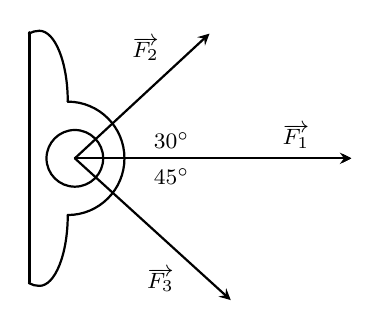
\begin{tikzpicture}[scale=0.9,font=\footnotesize,line join=round, line cap=round,>=stealth]
			\def\a{0.8}
			\def\b{1}
			%Vẽ các vật
			\draw[thick] (0:\a) arc (90:-90:{\a});
			\draw[thick] (0:\a) arc (0:90:{\a-0.4 and {\b} });
			\draw[thick] (-63.434:2.236*\a) arc (0:-90:{\a-0.4} and {\b});
			\draw [thick] (\a-\b+1.1,-\a) circle (\a-0.4);
			\draw [thick] (\a-\b+0.6,\b)  arc (90:120:{\a-0.5});
			\draw [thick] (\a-\b+0.6,-2*\a-\b)  arc (-90:-120:{\a-0.5});
			\draw [thick]  (\a-\b+0.46,-2*\a-\b+0.05)--(\a-\b+0.46,2*\a-0.62);
			%Vẽ các mũi tên
			\draw[->](\a-\b+1.1,-\a)--(4.8,-\a) node[above,pos=0.35]{$30^\circ$};
			\draw[->](\a-\b+1.1,-\a)--(4.8,-\a) node[above,pos=0.8, thick]{$\overrightarrow{F_1}$};
			\draw[->,thick](\a-\b+1.1,-\a)--(4.8,-\a) node[below,pos=0.35]{$45^\circ$};
			\draw[->, thick](\a-\b+1.1,-\a)--(2.8,1.2*\a) node[above left,pos=0.7]{$\overrightarrow{F_2}$};
			\draw[->, thick](\a-\b+1.1,-\a)--(3.1,-\a-2) node[below left,pos=0.7]{$\overrightarrow{F_3}$};
	\end{tikzpicture}}
	\loigiai{\immini{Chọn hệ trục tọa độ $Oxy$ như hình bên, $x$ và $y$ tính bằng Newton.\\
			Ta có $\overrightarrow{F_1}=(15;0)$.\\
			Vì $\left(\overrightarrow{F_1};\overrightarrow{F_2}\right)=30^\circ$ nên tọa độ $\overrightarrow{F_2}$ là $$\overrightarrow{F_2}=\left(6 \cos 30^\circ; 6 \sin 30^\circ \right)=(3 \sqrt{3};3).$$
			Vì $\left(\overrightarrow{F_1};\overrightarrow{F_3}\right)=45^\circ$ nên tọa độ $\overrightarrow{F_3}$ là $$\overrightarrow{F_3}=\left(8 \cos 45^\circ; -8 \sin 45^\circ \right)=(4 \sqrt{2};-4\sqrt{2}).$$}
		{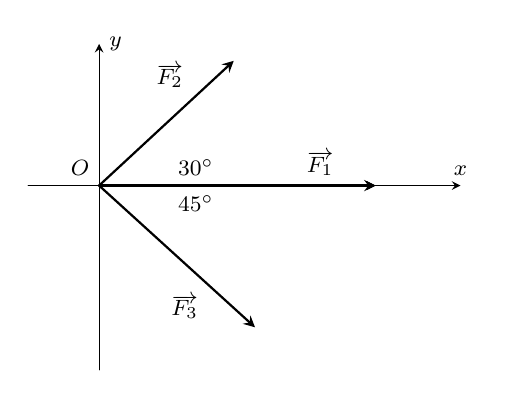
\begin{tikzpicture}[scale=0.9,font=\footnotesize,line join=round, line cap=round,>=stealth]
				\def\a{0.8}
				\def\b{1}
				%Vẽ trục tọa độ
				\draw[->](\a-\b+1.1-1,-\a)--(6,-\a) node[above, thick]{$x$};
				\draw[->](\a-\b+1.1,-\a-2.6)--(\a-\b+1.1,-\a+2) node[right, thick]{$y$};
				\draw (\a-\b+1.1,-\a) node [above left]{$O$};
				%Vẽ các mũi tên
				\draw[->](\a-\b+1.1,-\a)--(4.8,-\a) node[above,pos=0.35]{$30^\circ$};
				\draw[->](\a-\b+1.1,-\a)--(4.8,-\a) node[above,pos=0.8, thick]{$\overrightarrow{F_1}$};
				\draw[->,thick](\a-\b+1.1,-\a)--(4.8,-\a) node[below,pos=0.35]{$45^\circ$};
				\draw[->, thick](\a-\b+1.1,-\a)--(2.8,1.2*\a) node[above left,pos=0.7]{$\overrightarrow{F_2}$};
				\draw[->, thick](\a-\b+1.1,-\a)--(3.1,-\a-2) node[below left,pos=0.7]{$\overrightarrow{F_3}$};
		\end{tikzpicture}}	
		Do đó, lực $\overrightarrow{F}$ tổng hợp các lực tác động lên vật có tọa độ là 
		$$\overline{F}=\overrightarrow{F_1}+\overrightarrow{F_2}+\overrightarrow{F_3}=(15+3\sqrt{3}+4\sqrt{2};3-4\sqrt{2}).$$
		Độ lớn lực $\overrightarrow{F}$ tác động lên vật là 
		$$\left| \overrightarrow{F} \right| = \sqrt{\left(15+3\sqrt{3}+4\sqrt{2}\right)^2+\left(3-4\sqrt{2}\right)^2} \approx 26 \; \text{N}.$$
		Vậy lực tổng hợp tác động lên vật có độ lớn khoảng là $26$ N.}
\end{ex}

\Closesolutionfile{ans}
